\documentclass[12pt]{article}

\title{Activity 8: Arrays}
\author{Dr. Chris Mayfield}
\date{CS 149, Fall 2016}

%\ProvidesPackage{cspogil}

% fonts
\usepackage[utf8]{inputenc}
\usepackage[T1]{fontenc}
\usepackage{mathpazo}

% spacing
\usepackage[margin=2cm]{geometry}
\renewcommand{\arraystretch}{1.4}
\setlength{\parindent}{0pt}

% orphans and widows
\clubpenalty=10000
\widowpenalty=10000
\pagestyle{empty}

% figures and tables
\usepackage{graphicx}
\usepackage{multicol}
\usepackage{tabularx}
\usepackage{wrapfig}

% fixed-width columns
\usepackage{array}
\newcolumntype{L}[1]{>{\raggedright\let\newline\\\arraybackslash\hspace{0pt}}m{#1}}
\newcolumntype{C}[1]{>{\centering\let\newline\\\arraybackslash\hspace{0pt}}m{#1}}
\newcolumntype{R}[1]{>{\raggedleft\let\newline\\\arraybackslash\hspace{0pt}}m{#1}}

% include paths
\makeatletter
\def\input@path{{Models/}{../../Models/}}
\graphicspath{{Models/}{../../Models/}}
\makeatother

% colors
\usepackage[svgnames,table]{xcolor}
\definecolor{bgcolor}{HTML}{FAFAFA}
\definecolor{comment}{HTML}{007C00}
\definecolor{keyword}{HTML}{0000FF}
\definecolor{strings}{HTML}{B20000}

% table headers
\newcommand{\tr}{\bf\cellcolor{Yellow!10}}

% syntax highlighting
\usepackage{textcomp}
\usepackage{listings}
\lstset{
    basicstyle=\ttfamily\color{black},
    backgroundcolor=\color{bgcolor},
    numberstyle=\scriptsize\color{comment},
    commentstyle=\color{comment},
    keywordstyle=\color{keyword},
    stringstyle=\color{strings},
    columns=fullflexible,
    keepspaces=true,
    showlines=true,
    showstringspaces=false,
    upquote=true
}

% code environments
\newcommand{\java}[1]{\lstinline[language=java]{#1}}%[
\lstnewenvironment{javalst}{\lstset{language=java,backgroundcolor=}}{}
\lstnewenvironment{javabox}{\lstset{language=java,frame=single,numbers=left}\quote}{\endquote}

% PDF properties
\usepackage[pdftex]{hyperref}
\urlstyle{same}
\makeatletter
\hypersetup{
  pdftitle={\@title},
  pdfauthor={\@author},
  pdfsubject={\@date},
  pdfkeywords={},
  bookmarksopen=false,
  colorlinks=true,
  citecolor=black,
  filecolor=black,
  linkcolor=black,
  urlcolor=blue
}
\makeatother

% titles
\makeatletter
\renewcommand{\maketitle}{\begin{center}\LARGE\@title\end{center}}
\makeatother

% boxes [optional height]
\newcommand{\emptybox}[1][10em]{
\vspace{1em}
\begin{tabularx}{\linewidth}{|X|}
\hline\\[#1]\hline
\end{tabularx}}

% models
\newcommand{\model}[1]{\section{#1}\nopagebreak}
\renewcommand{\thesection}{Model~\arabic{section}}

% questions
\newcommand{\quest}[1]{\subsection*{Questions~ (#1)}}
\newcounter{question}
\newcommand{\Q}{\vspace{1em}\refstepcounter{question}\arabic{question}.~ }
\renewcommand{\thequestion}{\#\arabic{question}}

% sub-question lists
\usepackage{enumitem}
\setenumerate[1]{label=\alph*)}
\setlist{itemsep=1em,after=\vspace{1ex}}

% inline answers
\definecolor{answers}{HTML}{C0C0C0}
\newcommand{\ans}[1]{%
\ifdefined\Student
    \leavevmode\phantom{~~\textcolor{answers}{#1}}
\else
    ~~\textcolor{answers}{#1}
\fi}

% longer answers [optional height]
\newsavebox{\ansbox}
\newenvironment{answer}[1][4em]{
\nopagebreak
\begin{lrbox}{\ansbox}
\begin{minipage}[t][#1]{\linewidth}
\color{answers}
}{
\end{minipage}
\end{lrbox}
\ifdefined\Student
    \phantom{\usebox{\ansbox}}%
\else
    \usebox{\ansbox}%
\fi}


\begin{document}

\maketitle

Programs often need to store multiple values of the same type, such as a list of 1000 phone numbers or the names of your top 20 favorite songs.
Rather than create a separate variable for each one, we can store them together using an array.

% based on Model 1 of Activity 13 - TwoD Arrays by Helen Hu

\model{Array Syntax}

%An \emph{array} allows you to declare a collection of related variables (of the same type) at once.
Each value in an array is known as an \emph{element}.
The programmer must specify the \emph{length} of the array (the number of array elements).
Once the array is created, its length cannot be changed.

\begin{quote}
\begin{javalst}
String[] wordArray = {"hello", "world"};
System.out.println(wordArray[0]);            // outputs hello
System.out.println(wordArray.length);        // outputs 2

double[] numberArray = new double[365];
System.out.println(numberArray[0]);          // outputs 0.0
System.out.println(numberArray.length);      // outputs 365
\end{javalst}
\end{quote}

Array elements are accessed by \emph{index} number, starting at zero:

\begin{quote}
\begin{tabular}{cc}
\hline
\multicolumn{1}{|c|}{\java{"hello"}} &
\multicolumn{1}{ c|}{\java{"world"}} \\
\hline
\fs 0 & \fs 1 \\
\end{tabular}
\hspace{3em}
\begin{tabular}{ccC{4em}c}
\hline
\multicolumn{1}{|c|}{\java{0.0}} &
\multicolumn{1}{ c|}{\java{0.0}} &
\multicolumn{1}{ c|}{$\cdots$} &
\multicolumn{1}{ c|}{\java{0.0}} \\
\hline
\fs 0 & \fs 1 &   & \fs 364 \\
\end{tabular}
\end{quote}


\quest{15 min}


\Q Examine the results of the above code.

\begin{enumerate}
\item What is the index for the element \java{"world"}? \ans{1}
\item What is the length of the \java{wordArray}? \ans{2}
\item What is the length of the \java{numberArray}? \ans{365}
\item How would you access the last element of \java{numberArray}? \ans{\java{numberArray[364]}}
\end{enumerate}


\Q Now examine the syntax of the code.

\begin{enumerate}
\item What are three ways that square brackets [] are used? \ans{
1) To declare the type: {\tt String[]}.
2) To specify the length: {\tt double[365]}.
3) To access an element: {\tt wordArray[0]}.}

\item In contrast, how are curly braces {} used for an array?
\ans{To create an array with an initial set of values.}
\end{enumerate}


\begin{tabularx}{\linewidth}{|X|}
\hline
Array variables can be initialized without the \java{new} keyword: \\
~~~~~~~~\java{int[] picks = \{3, 5, 7, 2, 1\};} \\[-1ex]
~~~~~~~~\java{String[] names = \{"Grace", "Alan", "Tim"\};} \\[1ex]

However, if the variable is already declared, \java{new} is required: \\
~~~~~~~~\java{picks = new int[] \{3, 5, 7, 2, 1\};} \\[-1ex]
~~~~~~~~\java{names = new String[] \{"Grace", "Alan", "Tim"\};} \\
\hline
\end{tabularx}
\vspace{1ex}


\Q Write \emph{expressions} that create the following \java{new} arrays. (Do not declare variables.)

\begin{enumerate}

\item
\begin{tabular}{|C{3em}|C{3em}|C{3em}|C{3em}|C{3em}|C{3em}|}
\hline
0 & 14 & 1024 & 127 & 3 & 5521 \\
\hline
\end{tabular}

\vspace{1ex}
\ans{\tt new int[] \{0, 14, 1024, 127, 3, 5521\}}

\item 
\begin{tabular}{|C{3em}|C{3em}|C{3em}|C{3em}|C{3em}|C{3em}|C{3em}|}
\hline
3.23 & 1.52 & 4.23 & 32.5 & 2.45 & 5.23 & 3.33 \\
\hline
\end{tabular}

\vspace{1ex}
\ans{\tt new double[] \{3.23, 1.52, 4.23, 32.5, 2.45, 5.23, 3.33\}}

\end{enumerate}


\Q Write \emph{statements} that both declare and initialize variables for these \java{new} arrays.

\begin{enumerate}

\item
\begin{tabular}{|C{3em}|C{3em}|C{3em}|C{3em}|C{3em}|C{3em}|}
\hline
0 & 14 & 1024 & 127 & 3 & 5521 \\
\hline
\end{tabular}

\vspace{1ex}
\ans{\tt int[] a = \{0, 14, 1024, 127, 3, 5521\};}

\item 
\begin{tabular}{|C{3em}|C{3em}|C{3em}|C{3em}|C{3em}|C{3em}|C{3em}|}
\hline
3.23 & 1.52 & 4.23 & 32.5 & 2.45 & 5.23 & 3.33 \\
\hline
\end{tabular}

\vspace{1ex}
\ans{\tt double[] b = \{3.23, 1.52, 4.23, 32.5, 2.45, 5.23, 3.33\};}

\end{enumerate}


\Q What are the type and value for each of the four \emph{expressions} below?

\begin{javalst}
int[] a = {3, 6, 15, 22, 100, 0};
double[] b = {3.5, 4.5, 2.0, 2.0, 2.0};
String[] c = {"alpha", "beta", "gamma"};
\end{javalst}

\begin{enumerate}
\item \java{a[3] + a[2]}
\ans{Type: {\tt int}, Value: {\tt 37}}

\item \java{b[2] - b[0] + a[4]}
\ans{Type: {\tt double}, Value: {\tt 98.5}}

\item \java{c[1].charAt(a[0])}
\ans{Type: {\tt char}, Value: {\tt \qs{a}\qs}}

\item \java{a[4] * b[1] <= a[5] * a[0]}
\ans{Type: {\tt boolean}, Value: {\tt false}}
\end{enumerate}

\model{Array Diagrams}

Array elements are stored together in one contiguous block of memory. To show arrays in memory diagrams, we simply draw adjacent boxes.

\begin{center}
\java{int[] nums = \{10, 3, 7, -5\};}

\vspace{1ex}
%TODO need to model default values (see questions below)
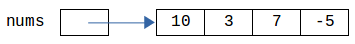
\includegraphics[width=225pt]{array-diagram1.png}
\end{center}


\quest{10 min}


\Q Draw a memory diagram for the following array declarations.

%TODO solution for array memory diagrams
\begin{enumerate}

\item
\begin{javalst}
int[] sizes = new int[5];
sizes[2] = 7;
\end{javalst}

\item
\begin{javalst}
double[] costs = new double[4];
costs[0] = 0.99;
\end{javalst}

\item
\begin{javalst}
String[] names = new String[3];
names[1] = "Anita";
\end{javalst}

\end{enumerate}


\Q What is the \emph{default} value for uninitialized array elements? (Hint: You should have no empty boxes in your memory diagrams above.)

\begin{answer}
Zero or equivalent value, depending on the data type.
For numeric types like {\tt int} and {\tt double}, the default is 0; for {\tt boolean}, it's {\tt false}; for {\tt char}, it's {\tt \qs{\bs u0000}\qs}; for reference types, it's {\tt null}.
\end{answer}


\Q Like strings, arrays are reference types. What is the \emph{value} of an array variable?

\begin{answer}
The memory location of the array. If you assign one array variable to another, you're only copying the reference, not the array itself.
\end{answer}


\Q Draw a memory diagram of the following array.
(Hint: You should have four arrows.)

\begin{javalst}
String[] greek = {"alpha", "beta", "gamma"};
\end{javalst}

\begin{answer}
%TODO string array memory diagram
\end{answer}

\model{Arrays and Loops}

The real power of arrays is the ability to process them using loops, i.e., performing the same task for multiple elements.

\begin{javalst}
    for (int i = 0; i < array.length; i++) {
       // ... process array[i] ...
    }
\end{javalst}

Here are two specific examples:

\begin{javalst}
    // set all of the elements of x to -1.0
    double[] x = new double[100];
    for (int i = 0; i < x.length; i++) {
        x[i] = -1.0;
    }
    // sum the elements of scores
    int sum = 0;
    for (int i = 0; i < scores.length; i++) {
        sum += scores[i];
    }
\end{javalst}


\quest{10 min}


\Q What is the value of \java{array} and \java{accumulator} at the end of the following code?
Trace the loop by hand in the space below.

\begin{javalst}
int[] array = {5, 26, 13, 12, 37, 15, 16, 4, 1, 3};
int accumulator = 0;
for (int i = 0; i < array.length; i++) {
    if (array[i] % 2 == 1 && i + 1 < array.length) {
        array[i] *= -1;
        accumulator += array[i+1];
    }
}
\end{javalst}

\begin{answer}[12em]
\begin{tabular}{|C{20pt}|C{40pt}|C{40pt}|}
\hline
i & array[i] & accum \\
\hline
\hline
0 & 5 & 0 \\
\hline
1 & 26 & 26 \\
\hline
2 & 13 & 26 \\
\hline
3 & 12 & 38 \\
\hline
4 & 37 & 38 \\
\hline
\end{tabular}
\hspace{20pt}
\begin{tabular}{|C{20pt}|C{40pt}|C{40pt}|}
\hline
i & array[i] & accum \\
\hline
\hline
5 & 15 & 53 \\
\hline
6 & 16 & 69 \\
\hline
7 & 4 & 69 \\
\hline
8 & 1 & 69 \\
\hline
9 & 3 & 72 \\
\hline
\end{tabular}
\hspace{20pt}
\begin{minipage}{175pt}
\begin{javalst}
array:
  { -5, 26, -13, 12, -37,
   -15, 16,   4, -1,   3}

accumulator:
  72
\end{javalst}
\end{minipage}
\end{answer}


\newpage

\Q \label{pairwiseMax}
Implement the following method that creates and returns a new array.

\begin{javalst}
/**
 * Return a new array containing the pairwise maximum value of
 * the arguments. For each subscript i, the return value at [i]
 * will be the larger of x[i] and y[i].
 *
 * @param x an array of double values
 * @param y an array of double values
 * @return pairwise max of x and y
 */
public static double[] pairwiseMax(double[] x, double[] y) {
\end{javalst}

\vspace{-3ex}
\begin{answer}[11.3em]
\begin{javaans}
    double[] z = new double[x.length];
    for (int i = 0; i < x.length; i++) {
        if (x[i] > y[i]) {
            z[i] = x[i];
        } else {
            z[i] = y[i];
        }
    }
    return z;
\end{javaans}
\end{answer}

\begin{javalst}
}
\end{javalst}


\Q \label{finalGrade}
Implement the following method that reads through two integer arrays.

\begin{javalst}
/**
 * Computes the final average grade for a student. The labs are
 * worth 40% and the exams are worth 60%. All scores range from
 * 0 to 100, inclusive.
 *
 * @param labs the student's lab scores
 * @param exams the student's exam scores
 * @return weighted average of all scores
 */
public static double finalGrade(int[] labs, int[] exams) {
\end{javalst}

\vspace{-3ex}
\begin{answer}[13.7em]
\begin{javaans}
    int labSum = 0;
    for (int score : labs) {
        labSum += score;
    }
    int examSum = 0;
    for (int score : exams) {
        examSum += score;
    }
    double labGrade = 1.0 * labSum / labs.length;
    double examGrade = 1.0 * examSum / exams.length;
    return 0.40 * labGrade + 0.60 * examGrade;
\end{javaans}
\end{answer}

\begin{javalst}
}
\end{javalst}


\end{document}
